\documentclass{article}
\usepackage{amsmath,amssymb}
\usepackage{tikz}
\usetikzlibrary{arrows.meta,positioning,calc,shapes.geometric}
\pagestyle{empty}
\begin{document}
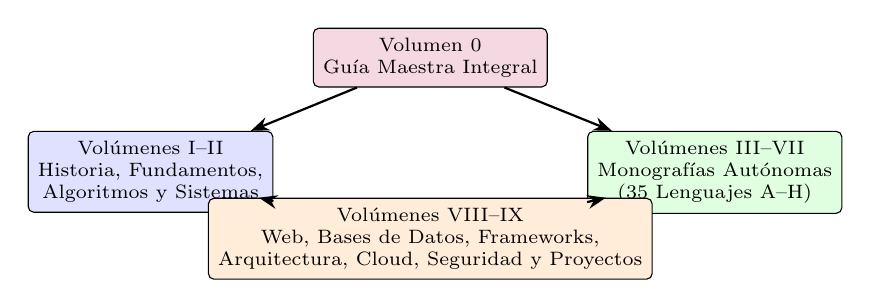
\begin{tikzpicture}
\tikzset{node distance=0.55cm and 0.5cm, every node/.style={font=\scriptsize, draw, rounded corners=2pt, align=center, inner sep=3.5pt}}
\node (v0) [fill=purple!15] {Volumen 0\\Guía Maestra Integral};
\node (v12) [below left=of v0, fill=blue!12] {Volúmenes I–II\\Historia, Fundamentos,\\Algoritmos y Sistemas};
\node (v37) [below right=of v0, fill=green!12] {Volúmenes III–VII\\Monografías Autónomas\\(35 Lenguajes A–H)};
\node (v89) [below=1.4cm of v0, fill=orange!15] {Volúmenes VIII–IX\\Web, Bases de Datos, Frameworks,\\Arquitectura, Cloud, Seguridad y Proyectos};
\draw[-Stealth, thick] (v0) -- (v12);
\draw[-Stealth, thick] (v0) -- (v37);
\draw[-Stealth, thick] (v12) -- (v89);
\draw[-Stealth, thick] (v37) -- (v89);
\end{tikzpicture}
\end{document}
